\documentclass[10pt]{beamer}

\usepackage[UKenglish]{babel}
\usepackage{hyperref}
\usepackage[utf8]{inputenc}
\usepackage[backend=bibtex,style=ieee,maxbibnames=99]{biblatex}
\usepackage[uni,footuni,headframelogo]{./unirostock/beamerthemeRostock}
\usepackage{scrhack} %Fix for older packages

\title{IuK-Blockchain}
\subtitle{Progress report}
\author{\textsc{Robert Kohlen}\newline\textsc{Richard Dabels}\newline\textsc{Maximilian Jung}\newline\textsc{Daniel Decker}\newline\textsc{Nis Meinert}\newline\textsc{Hannes Hagen}}
\date{11.05.2018}
\footinstitute{Institut für Informatik}

\addbibresource{./references.bib}

\begin{document}

\begin{frame}
	\titlepage
\end{frame}

\begin{frame}{Task}
	\begin{itemize}
		\item Develop a private blockchain to use at the IuK chair
		\item Implement an example scenario to:
		\begin{itemize}
			\item Verify the autenticity of documents with the help of blockchains
			\item A way to add documents or hashes of documents to the blockchain
		\end{itemize}
	\end{itemize}
\end{frame}

\begin{frame}{Work divided into groups}
	\begin{itemize}
		\item Blockchain / Ethereum (4 persons)
		\item Web interface (3 persons)
	\end{itemize}
\end{frame}

\begin{frame}{Blockchain - from scratch}
	\begin{itemize}
		\item Easy way to get started thanks to lots of web tutorials
		\item High flexibility
		\item High learning effect
		\item Lots of work on the fundamentals
		\item Distributed systems are hard to debug
	\end{itemize}
\end{frame}

\begin{frame}{Blockchain - existing framework}
	\begin{itemize}
		\item Already tested by many people, thus might be less error-prone
		\item Faster progress on the real task
		\item i.e. implementation called go-ethereum provides way to setup private blockchains
	\end{itemize}
\end{frame}

\begin{frame}{Schedule}
	\begin{itemize}
		\item 4 weeks: Planning
			\begin{itemize}
				\item Use existing framework or implement own blockchain system
				\item Specification per group
			\end{itemize}
		\item 4 weeks: Implementation
			\begin{itemize}
				\item Implementation of blockchain and/or smart contracts
				\item Implementation of web interface
			\end{itemize}
		\item 4 weeks: Setup and testing
			\begin{itemize}
				\item Setup of servers (AWS?)
				\item Testing of the system
			\end{itemize}
	\end{itemize}
\end{frame}

\begin{frame}{Web interface}
	\begin{itemize}
		\item User interface to interact with blockchain:
			\begin{itemize}
				\item Add documents to blockchain
				\item Verify documents on blockchain
			\end{itemize}
	\end{itemize}
\end{frame}

\begin{frame}{Web interface}
	\begin{figure}
		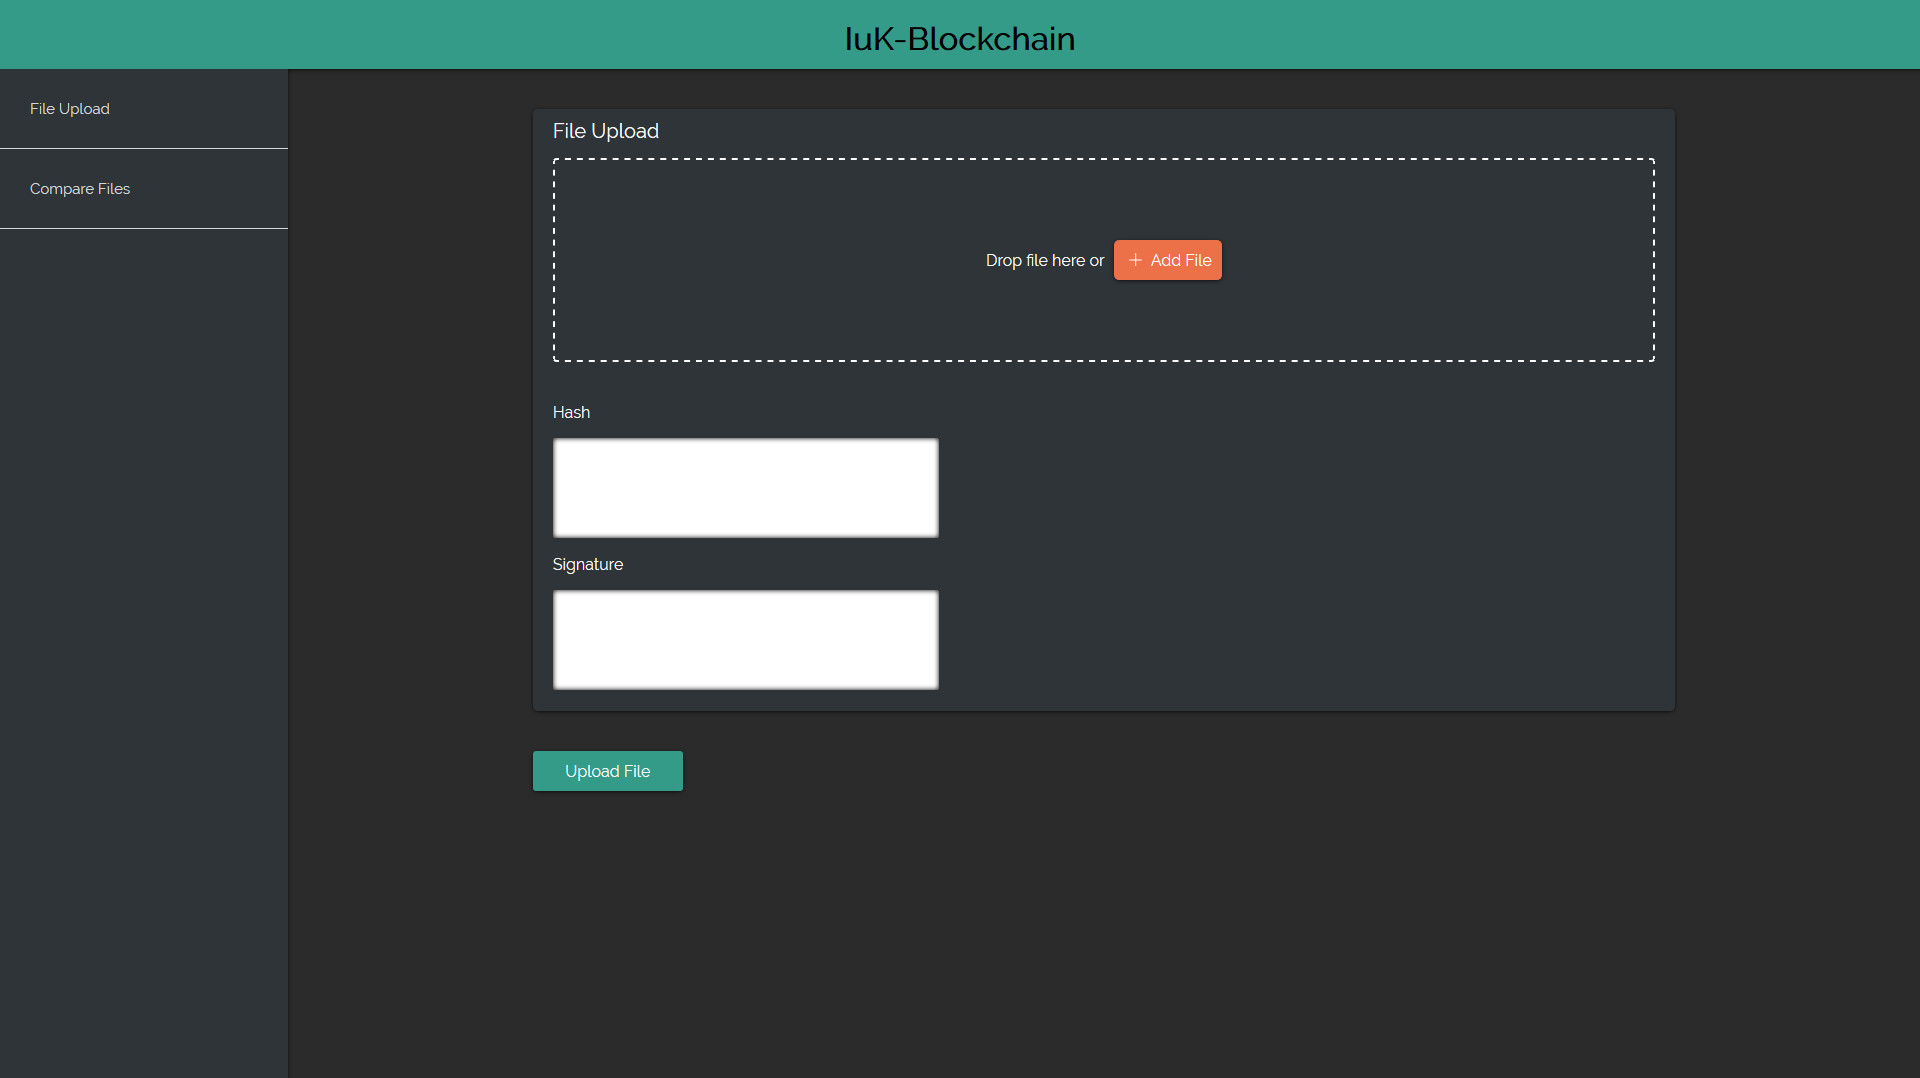
\includegraphics[width=1\textwidth]{images/GUI.jpg}
	\end{figure}
\end{frame}

%\begin{frame}[allowframebreaks]{References}
%Reduce URL font size
%\renewcommand{\UrlFont}{\small\rmfamily}
%\printbibliography
%\end{frame}

\end{document}
